\mysubsection{Lydia Friedrich}{Papierprototyp}

\begin{figure}[!htbp]%[htbp]
	\centering
		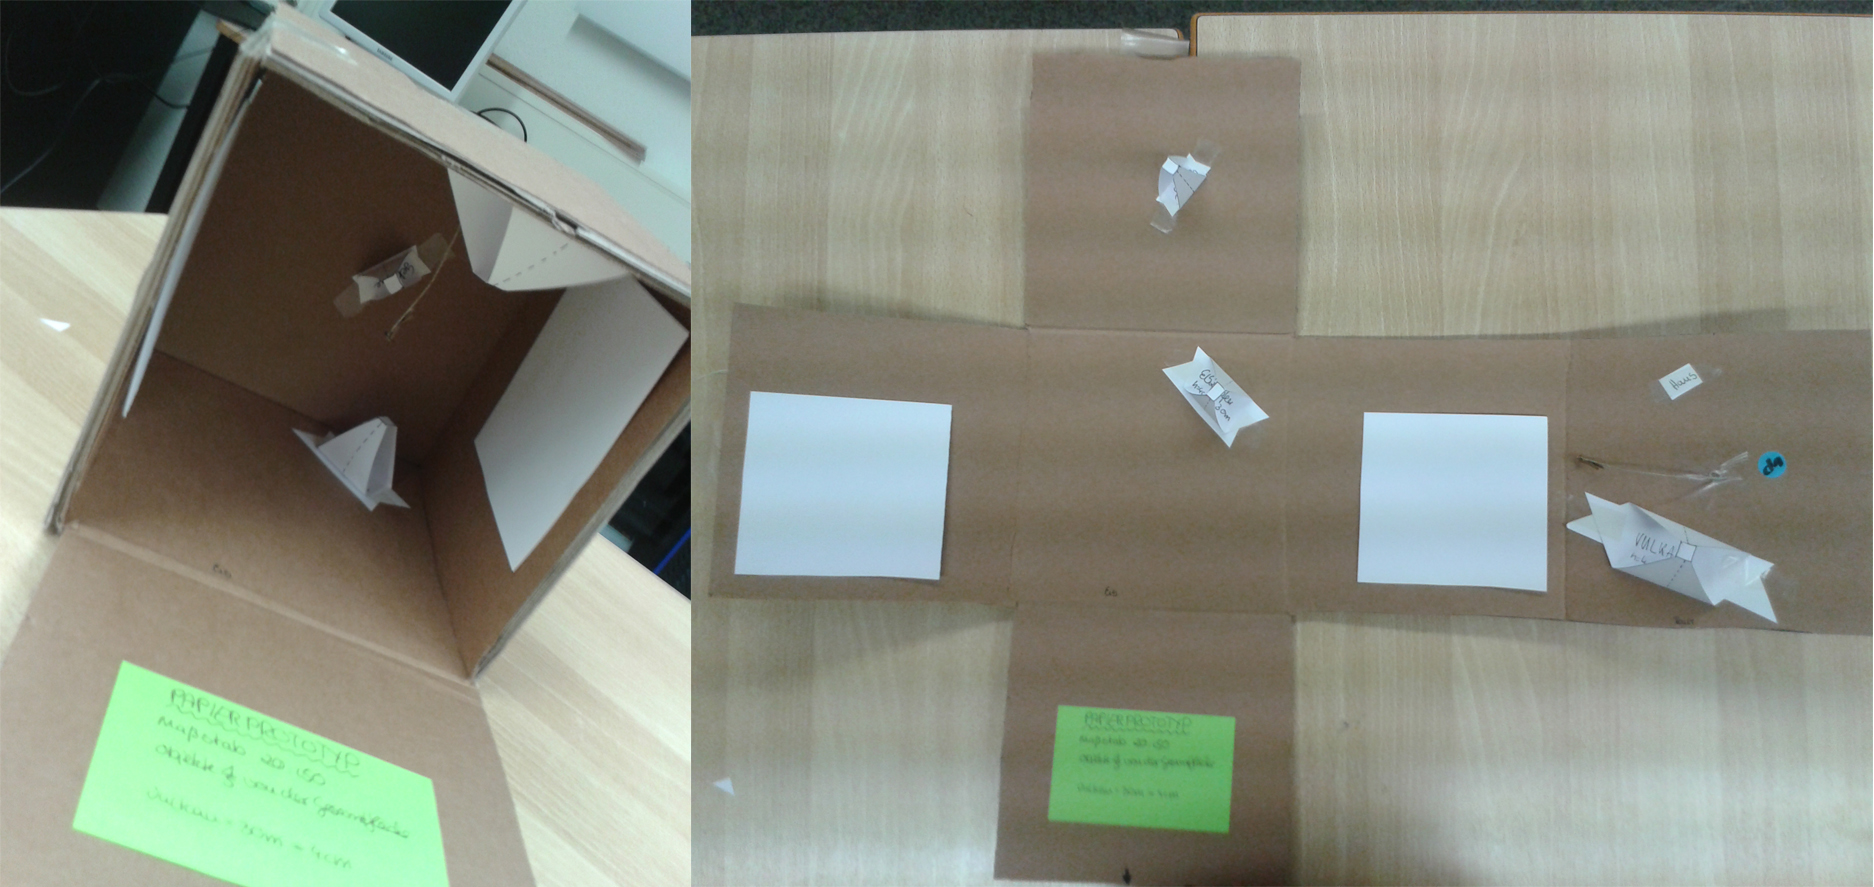
\includegraphics[width=0.9\textwidth]{images/Prototyp}
	\caption{Papierprototyp}
	\label{fig:Papierprototyp}
\end{figure}

Um einen ersten Überblick über die Komplexität der Spielwelten zu erhalten, wird ein Papierprototyp im Maßstab 20:150 und einigen Objekten auf den Innenseiten des Würfels mit Pappe umgesetzt. Versuche ergeben, dass eine Größe von 200x200 m, besser für eine Weltenfläche geeignet ist, als eine Größe von nur 150x150 m. Deshalb sollte man im Vornherein, zeitgleich zur Erstellung des Papierprotoypen einen Tiefeneindrucktest durchführen, um die Vergleichbarkeit der optischen und tatsächlichen Wahrnehmung möglich zu machen. Es zeigt sich, dass der Abstand des Spielers im Würfel zu den Welten und dessen herausragenden Objekten, eine entscheidene Rolle für einen angenehmen stereoskopischen Wahrnehmungseindruck des Spielers spielt. Zudem kann durch eine Kombination des Papierprototypens und einem Tiefeneindrucktest die Größe der Objekte auf den Welten und deren Abstand zur Position des Spielers bestimmt werden. Die Größe der Objekte wird auf 1:5 der Weltenreite festgelegt.